\chapter{Costruzione di un parser da una grammatica}
Individuiamo due passaggi per costruire un parser da una grammatica:
\begin{enumerate}
  \item la grammatica non deve essere ambigua;
    \begin{lstlisting}[language=Java, caption={Una grammatica non ambigua}]
    Exp ::= Mul | Exp '+' Mul
    Mul ::= Atom | Mul '*' Atom
    Atom ::= Num | '(' Exp ')'
    Num ::= '0' | '1'
    \end{lstlisting}
  \item per ogni token di input, il parser dever sceltiere una
    produzione unica da usare per l'albero \emph{parse} corretto.
\end{enumerate}

\paragraph{Problemi:}
\begin{itemize}
  \item i token sono letti dal parser da sinsitra a destra;
  \item nella più semplice delle ipotesi, il parser è a conoscenza
    solo del token successivo (\emph{lookahead token});
  \item un parser con un \emph{lookahead token} non è in grado di
    scegliere la giusta produzione per la grammatica di cui sopra.
\end{itemize}

\section{Come costruire un parser da una grammatica}
\begin{lstlisting}[language=Java, caption={Una grammatica non ambigua}]
  Exp ::= Mul | Exp '+' Mul
  Mul ::= Atom | Mul '*' Atom
  Atom ::= Num | '(' Exp ')'
  Num ::= '0' | '1'
\end{lstlisting}
Quindi un parser con \textbf{un} \emph{lookahead token} non può essere
costruito per la grammatica di cui sopra.
\paragraph{Controesempio:}
Se il primo lookahead token è un numero, allora entrambe le produzioni di
\emph{Exp} potrebbero funzionare.
A seconda del secondo lookahead token $t$:
\begin{itemize}
  \item la produzione ($Exp$,$Mul$) è usata se $t$ è $'*'$ oppure la fine
    dello stream di input;
  \item la produzione ($Exp$,$Exp$ $'+'$ $Mul$) è usata se $t='+'$.
\end{itemize}

\subparagraph{Osservazioni:}
Per costruire un albero \emph{parse}, la produzione ($Exp$,$Mul$) deve essere
usata, inoltre quando le produzioni di $Exp$ sono usate consecutivamente,
vengono ottenute stringhe della forma seguente: $Mul$, oppure $Mul$ seguita
dalla stringa $'+'Mul$ ripetuta una o più volte.

\begin{lstlisting}[language=Java, caption={Grammatica rivisitata a seguito delle osservazioni precedenti}]
  Exp ::= Mul | AddSeq
  AddSeq ::= '+' Mul | '+' Mul AddSeq
  Mul ::= Atom | Mul '*' Atom
  Atom ::= Num | '(' Exp ')'
  Num ::= '0' | '1'
\end{lstlisting}

\paragraph{Considerazioni sulla trasformazione della grammatica}
La grammatica è equivalente alla precedente, ma quando si costruisce un albero
\emph{parse} sappiamo che un nodo $Exp$ deve sempre avere un figlio $c$ a
sinistra etichettato da $Mul$ dopo che l'albero \emph{parse} con radice $c$ è
stato costruito, quindi la produzione corretta è ($Exp$, $Mul$ $AddSeq$) se
il token \emph{lookahead} è $'+'$;
altrimenti la produzione è ($Exp$,$Mul$): un nodo $AddSeq$ deve sempre avere un
figlio a sinistra $c_1$ etichettato da $'+'$, seguito da un figlio $c_2$
etichettato da $Mul$.

Dopo che l'albero con radice $c_2$  è costruito, la produzione corretta se
il token \emph{lookahead}$='+'$ è: ($AddSeq$, $'+'$ $Mul$ $AddSeq$), altrimenti
la produzione è ($AddSeq$, $'+'$ $Mul$).

\begin{lstlisting}[language=Java, caption={Soluzione completa}]
  Exp ::= Mul | AddSeq
  AddSeq ::= '+' Mul | '+' Mul AddSeq
  Mul ::= Atom | Atom MulSeq
  MulSeq ::= '*' Atom | '*' Atom MulSeq
  Atom ::= Num | '(' Exp ')'
  Num ::= '0' | '1'
\end{lstlisting}

\begin{figure}[H]
\caption{Parse tree per "1+1*1"}
\centering\resizebox{.5\textwidth}{!}{%
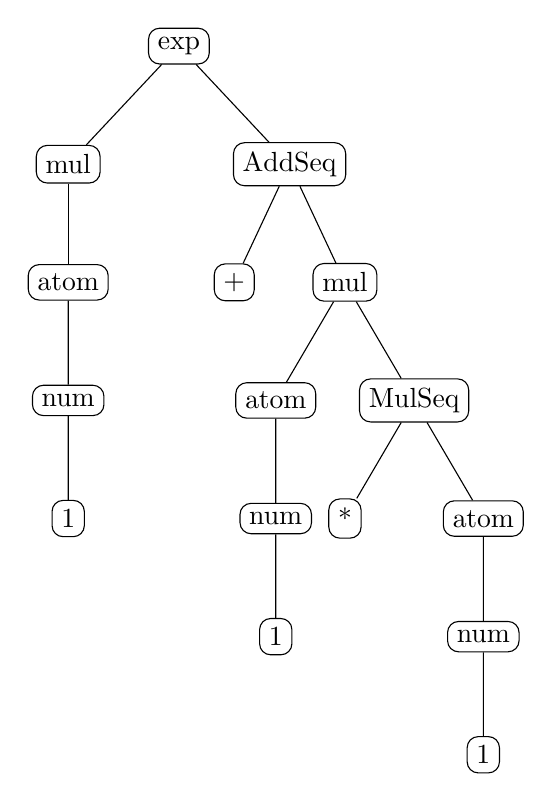
\begin{tikzpicture}[%
  level 1/.style = {sibling distance=8em},   % <-- added
  level 2/.style = {sibling distance=4em},    % <-- added
  level 3/.style = {sibling distance=5em},    % <-- added
  every node/.style = {
    shape=rectangle,
    rounded corners,
    draw,
    align=center
  }]
  \node {exp}
    child { node {mul}
      child { node {atom}
        child { node {num}
          child { node {1} }
        }
      }
    }
    child { node {AddSeq}
      child { node {+} }
      child { node {mul}
        child { node {atom}
          child { node {num}
            child { node {1} }
          }
        }
        child { node {MulSeq}
          child { node {*} }
          child { node {atom}
            child { node {num}
              child { node {1} }
            }
          }
        }
      }
    };
\end{tikzpicture}}\end{figure}

\section{Grammatiche EBNF}
La notazione \textbf{BNF} estende la notazione postfissa con gli operatori:
$*,+,?$.
La grammatica precedente può essere trasformata in una grammatica più semplice
utilizzando la notazione \textbf{EBNF}.

\begin{lstlisting}[language=Java, caption={Soluzione completa utilizando la gammatica ENBNF}]
  Exp ::= Mul | ('+' Mul)*
  Mul ::= Atom ('*' Atom)*
  Atom ::= Num | '(' Exp ')'
  Num ::= '0' | '1'
\end{lstlisting}

\subsection{Da una grammatica ad un parser top-down}
Per semplicità consideriamo solamente il problema del riconoscimento del
linguaggio, \textbf{top-down} significa che il \emph{parse tree} è costruito
dalla radice, l'albero di generazione sarà considerato nei laboratori.

\paragraph{Assunzioni sul tokenizer}
Il tokenizer definisce le procedure seguenti:
\begin{itemize}
  \item \textit{nextToken()}: la lettura del successivo \emph{lookahead token};
  \item \textit{tokenType()}: il tipo del token corrente;
  \item \textit{checkTokenType()}: il tipo del token corrente è controllatom
    un eccezione viene sollevata se il controllo fallisce, altrimenti viene
    letto il token successivo.
\end{itemize}

\subparagraph{Linee guida}
Il codice del parser proviene direttamente dalla grammatica, struttura
ricorsiva inclusa, il parser consiste in una procedura principale insieme ad
una procedura per ogni simbolo non terminale della grammatica.

\begin{lstlisting}[language=Java, caption={Pseudocodice detivara dalla grammatica EBNF precedente}]
parse(){
  nextToken()
  parseExp()
  checkTokenType(EOS)
}
parseExp(){
  parseMul()
  while(tokenType()==ADD){
    nextToken()
    parseMul()
  }
}
parseMul(){
  parseAtom()
  while(tokenType()==MUL){
    nextToken()
    parseAtom()
  }
}
parseAtom(){
  if(tokenType()==OPEN_PAR){
    nextToken()
    parseExp()
    checkTokenType(CLOSE_PAR)
  }
  else
    checkTokenType(NUM)
  nextToken()
}
\end{lstlisting}

\subsubsection{Grammatica EBNF per operatori con associatività a destra}
\begin{lstlisting}[language=Java, caption={Grammatica non ambigua}]
  // * con precedenza maggiore, sia + che * sono associativi a destra
  Exp ::= Mul | Mul '+' Exp
  Mul ::= Atom | Atom '*' Mul
  Atom ::= Num | '(' Exp ')'
  Num ::= '0' | '1'
\end{lstlisting}
\begin{lstlisting}[language=Java, caption={Grammatica EBNF equivalente}]
  Exp ::= Mul | ('+' Exp)?
  Mul ::= Atom ('*' Mul)?
  Atom ::= Num | '(' Exp ')'
  Num ::= '0' | '1'
\end{lstlisting}

\begin{lstlisting}[language=Java, caption={Pseudocodice derivato dalla grammatica EBNF precedente}]
parse(){
  nextToken()
  parseExp()
  checkTokenType(EOS)
}
parseExp(){
  parseMul()
  if(tokenType()==ADD){
    nextToken()
    parseExp()
  }
}
parseMul(){
  parseAtom()
  if(tokenType()==MUL){
    nextToken()
    parseMul()
  }
}
parseAtom(){
  if(tokenType()==OPEN_PAR){
    nextToken()
    parseExp()
    checkTokenType(CLOSE_PAR)
  }
  else
    checkTokenType(NUM)
  nextToken()
}
\end{lstlisting}

